\documentclass[11pt,aspectratio=169]{beamer}
\usetheme{Madrid}
\usecolortheme{dolphin}
\usepackage[utf8]{inputenc}
\usepackage{tikz}
\usetikzlibrary{positioning, arrows.meta, calc}
\usepackage{booktabs}
\usepackage{helvet}
\usepackage{array}
\usepackage{colortbl}
\usepackage{xcolor}
\usepackage{amssymb}
\usepackage{adjustbox}

\title[Quantitative Project Management]{Quantitative Project Management}
\subtitle{MGT 207}
\author{}
\date{10/8/26}

\newcommand{\cpmnode}[9]{
\node[draw, inner sep=0pt, thick, #1] (#2) at #3 {
  \renewcommand{\arraystretch}{1.2}
  \begin{tabular}{>{\centering\arraybackslash}p{0.65cm}|>{\centering\arraybackslash}p{0.65cm}}
    #4 & #5 \\ \hline
    \textbf{#6} & #7 \\ \hline
    #8 & #9
  \end{tabular}
};
}

\begin{document}

\begin{frame}
    \titlepage
\end{frame}

\begin{frame}{Idea Behind Formalizing PM}
    \begin{itemize}[<+->]
        \item \textbf{Learn the ``Physics'' of Project Management}
        \begin{itemize}
            \item The goal of learning these mathematical models (CPM, PERT) isn't just to help you win today's simulation game. 
            \item It is to teach you the underlying mechanics of how projects behave. Without understanding these foundational physics, it is very hard to manage complex projects competently without resorting to superficial guesswork.
        \end{itemize}
        \item \textbf{Use structure to combat scale and complexity}
        \item \textbf{Make future possibilities more predictable}, foresee problems, develop contingency plans
        \item \textbf{Forces us to confront things that are hard to think about in detail}
        \begin{itemize}
            \item Helpful even when the details don't unfold as expected
            \item Eisenhower: ``The plan is nothing. Planning is everything.''
        \end{itemize}
    \end{itemize}
\end{frame}

\begin{frame}{Setting Up Project Norms}
    \begin{itemize}[<+->]
        \item \textbf{Determine how the project will operate day to day}
        \begin{itemize}
            \item Set norms for meetings, updates, communication
            \item Establish official processes for logging, reviewing, updating progress on issues
            \item Set norms and escalation procedures for disagreements and unresolved issues
        \end{itemize}
        \item \textbf{Important questions:}
        \begin{itemize}
            \item What do we do when we encounter a new problem?
            \item Who do we go to for help making decisions?
            \item How do we check progress on a known issue?
        \end{itemize}
    \end{itemize}
\end{frame}

\begin{frame}{Overview}
    \begin{enumerate}[I.]
        \item \textbf{Project scheduling with known activity times}
        \begin{itemize}
            \item Example
            \item CPM approach
        \end{itemize}
        \vspace{1em}
        \item \textbf{Project Crashing}
        \begin{itemize}
            \item Heuristic approach
        \end{itemize}
        \vspace{1em}
        \item \textbf{Project scheduling with uncertain activity times}
        \begin{itemize}
            \item PERT approach
            \item Simulation approach
        \end{itemize}
        \vspace{1em}
        \item \textbf{Case study discussion}
    \end{enumerate}
\end{frame}

\begin{frame}{Product Launch at AeroTech Solutions}
    \small
    AeroTech Solutions has designed a revolutionary new autonomous delivery drone targeted at commercial logistics companies. R\&D and core design are complete. All that remains is to plan the manufacturing ramp-up and the global marketing campaign. The company has identified 9 key activities and the estimated costs for the project launch. How should AeroTech schedule these activities to hit the market in the shortest possible time?
    
    \vspace{0.5em}
    \begin{adjustbox}{max width=\linewidth, max height=0.6\textheight, center}
    \begin{tabular}{llccc}
        \toprule
        \textbf{Activity} & \textbf{Activity Description} & \textbf{Immediate} & \textbf{Activity Time} & \textbf{Normal Cost} \\
        & & \textbf{Predecessor} & \textbf{(weeks)} & \\
        \midrule
        A & Conduct market analysis & -- & 6 & \$240,000 \\
        B & Secure manufacturing facilities & A & 4 & \$300,000 \\
        C & Hire production managers & A & 3 & \$150,000 \\
        D & Procure raw materials & B & 3 & \$540,000 \\
        E & Hire \& train assembly team & B, C & 10 & \$900,000 \\
        F & Manufacture pilot units (prototypes) & D, E & 2 & \$300,000 \\
        G & Scale to full production & F & 6 & \$1,350,000 \\
        H & Develop marketing strategy & B & 6 & \$450,000 \\
        I & Execute global launch campaign & H, F & 8 & \$1,050,000 \\
        \midrule
        & & \textbf{Total} & \textbf{48} & \\
        \bottomrule
    \end{tabular}
    \end{adjustbox}
\end{frame}

\begin{frame}{Construction of a Network Diagram}
    \textbf{Given:}
    \begin{enumerate}[(1)]
        \item list of all activities
        \item precedence relationships
        \item estimates of time and cost for each activity
    \end{enumerate}
    \vspace{1em}
    \textbf{We are able to construct a network diagram where:}
    \begin{enumerate}[(1)]
        \item each \underline{node} represents an \underline{activity}
        \item each \underline{arc} represents the precedence relationship between two activities
        \item there is a (dummy) starting node ST and a (dummy) finishing node FIN
    \end{enumerate}
\end{frame}

\begin{frame}{Scheduling Calculations}
    After creating a network of a project, the next step in the CPM is to determine the earliest time that each activity in the network can start and finish. We determine these by what is called a \textcolor{blue}{forward pass}.
    
    \vspace{1em}
    \textbf{A. Notation}
    \begin{itemize}
        \item $t_k$ = estimate of the mean duration time of activity $k$
        \item $ES_k$ = \textcolor{blue}{earliest start} time for activity $k$
        \item $EF_k$ = \textcolor{blue}{earliest finish} time for activity $k$
        \item $LS_k$ = \textcolor{blue}{latest} allowable \textcolor{blue}{start} time for activity $k$
        \item $LF_k$ = \textcolor{blue}{latest} allowable \textcolor{blue}{finish} time for activity $k$
    \end{itemize}
    \vspace{1em}
    \begin{center}
    \begin{tabular}{|c|c|}
    \hline
    $ES_k$ & $EF_k$ \\ \hline
    $k$ & $t_k$ \\ \hline
    $LS_k$ & $LF_k$ \\ \hline
    \end{tabular}
    \end{center}
\end{frame}

\begin{frame}{Forward Pass}
    \textbf{B. Rules}
    \vspace{0.5em}
    
    \textbf{(1) Forward Pass (ES, EF)}
    
    \underline{Step 1:} for START node, set \textcolor{blue}{$ES_{start} = 0$}
    
    \vspace{1em}
    \underline{Step 2:} an arbitrary activity $k$ is assumed to start as soon as all of its predecessor activities are completed. This may be written as:
    
    $$ES_k = \text{largest EF of activity } k\text{'s predecessors} = \max_{j \in k\text{'s immed. pred.}} \{EF_j\}$$
    $$ = \text{the earliest possible time to start activity } k$$
    
    \vspace{1em}
    \underline{Step 3:} the earliest possible finish time of activity $k$ is the sum of its earliest start time and the estimated activity time.
    
    $$EF_k = ES_k + t_k$$
\end{frame}

\begin{frame}{Forward Pass (Step-by-Step)}
    \begin{adjustbox}{max width=\linewidth, max height=0.75\textheight, center}
    \begin{tikzpicture}[
        myarrow/.style={-Latex, thick},
        x=2.5cm, y=1.8cm
    ]
    % Coordinates
    \coordinate (posST) at (0, 1);
    \coordinate (posA)  at (0, -0.5);
    \coordinate (posB)  at (1, 1.2);
    \coordinate (posC)  at (1, -1.2);
    \coordinate (posH)  at (2, 1.8);
    \coordinate (posD)  at (2, 0);
    \coordinate (posE)  at (2, -1.8);
    \coordinate (posI)  at (4, 1.5);
    \coordinate (posF)  at (3, 0.5);
    \coordinate (posG)  at (4, -0.5);
    \coordinate (posFIN) at (5, 1);

    % ST
    \cpmnode{fill=white}{ST}{(posST)}{\only<1->{0}}{\only<1->{0}}{ST}{0}{}{}
    
    % A
    \cpmnode{fill=white}{A}{(posA)}{\only<2->{0}}{\only<2->{6}}{A}{6}{}{}
    \draw[myarrow] (ST) -- (A);

    % B & C
    \cpmnode{fill=white}{B}{(posB)}{\only<3->{6}}{\only<3->{10}}{B}{4}{}{}
    \cpmnode{fill=white}{C}{(posC)}{\only<3->{6}}{\only<3->{9}}{C}{3}{}{}
    \draw[myarrow] (A) -- (B);
    \draw[myarrow] (A) -- (C);

    % H & D & E
    \cpmnode{fill=white}{H}{(posH)}{\only<4->{10}}{\only<4->{16}}{H}{6}{}{}
    \cpmnode{fill=white}{D}{(posD)}{\only<4->{10}}{\only<4->{13}}{D}{3}{}{}
    \cpmnode{fill=white}{E}{(posE)}{\only<4->{10}}{\only<4->{20}}{E}{10}{}{}
    \draw[myarrow] (B) -- (H);
    \draw[myarrow] (B) -- (D);
    \draw[myarrow] (B) -- (E);
    \draw[myarrow] (C) -- (E);

    % F
    \cpmnode{fill=white}{F}{(posF)}{\only<5->{20}}{\only<5->{22}}{F}{2}{}{}
    \draw[myarrow] (D) -- (F);
    \draw[myarrow] (E) -- (F);

    % I & G
    \cpmnode{fill=white}{I}{(posI)}{\only<6->{22}}{\only<6->{30}}{I}{8}{}{}
    \cpmnode{fill=white}{G}{(posG)}{\only<6->{22}}{\only<6->{28}}{G}{6}{}{}
    \draw[myarrow] (H) -- (I);
    \draw[myarrow] (F) -- (I);
    \draw[myarrow] (F) -- (G);

    % FIN
    \cpmnode{fill=white}{FIN}{(posFIN)}{\only<7->{30}}{\only<7->{30}}{FIN}{0}{}{}
    \draw[myarrow] (I) -- (FIN);
    \draw[myarrow] (G) -- (FIN);
    \end{tikzpicture}
    \end{adjustbox}
\end{frame}

\begin{frame}{Backward Pass}
    \textbf{(2) Backward Pass (LS, LF)}
    \vspace{0.5em}
    
    \underline{Step 1:} LF of FINISH node is set equal to its earliest finish time as computed in the forward pass computations: $LF_{FIN} = EF_{FIN}$
    
    \vspace{1em}
    \underline{Step 2:} the latest allowable finish time for activity $k$ without delaying the entire project is the smallest (or earliest) of the latest allowable start times of its successor activities.
    
    $$LF_k = \text{smallest LS of } k\text{'s successors} = \min_{j \in k\text{'s immed. succ.}} \{LS_j\}$$
    $$= \text{latest allowable finish time for activity } k \text{ without affecting proj. completion}$$
    
    \vspace{1em}
    \underline{Step 3:} the latest allowable start time for activity $k$ without delaying the entire project is its latest allowable finish time minus the estimated activity time.
    
    $$LS_k = LF_k - t_k$$
\end{frame}

\begin{frame}{Backward Pass (Step-by-Step)}
    \begin{adjustbox}{max width=\linewidth, max height=0.75\textheight, center}
    \begin{tikzpicture}[
        myarrow/.style={-Latex, thick},
        x=2.5cm, y=1.8cm
    ]
    % Coordinates
    \coordinate (posST) at (0, 1);
    \coordinate (posA)  at (0, -0.5);
    \coordinate (posB)  at (1, 1.2);
    \coordinate (posC)  at (1, -1.2);
    \coordinate (posH)  at (2, 1.8);
    \coordinate (posD)  at (2, 0);
    \coordinate (posE)  at (2, -1.8);
    \coordinate (posI)  at (4, 1.5);
    \coordinate (posF)  at (3, 0.5);
    \coordinate (posG)  at (4, -0.5);
    \coordinate (posFIN) at (5, 1);

    % Forward pass data is static here
    \cpmnode{fill=white}{FIN}{(posFIN)}{30}{30}{FIN}{0}{\only<1->{30}}{\only<1->{30}}
    
    \cpmnode{fill=white}{I}{(posI)}{22}{30}{I}{8}{\only<2->{22}}{\only<2->{30}}
    \cpmnode{fill=white}{G}{(posG)}{22}{28}{G}{6}{\only<2->{24}}{\only<2->{30}}
    
    \cpmnode{fill=white}{F}{(posF)}{20}{22}{F}{2}{\only<3->{20}}{\only<3->{22}}
    \cpmnode{fill=white}{H}{(posH)}{10}{16}{H}{6}{\only<3->{16}}{\only<3->{22}}
    
    \cpmnode{fill=white}{D}{(posD)}{10}{13}{D}{3}{\only<4->{17}}{\only<4->{20}}
    \cpmnode{fill=white}{E}{(posE)}{10}{20}{E}{10}{\only<4->{10}}{\only<4->{20}}
    
    \cpmnode{fill=white}{B}{(posB)}{6}{10}{B}{4}{\only<5->{6}}{\only<5->{10}}
    \cpmnode{fill=white}{C}{(posC)}{6}{9}{C}{3}{\only<5->{7}}{\only<5->{10}}
    
    \cpmnode{fill=white}{A}{(posA)}{0}{6}{A}{6}{\only<6->{0}}{\only<6->{6}}
    \cpmnode{fill=white}{ST}{(posST)}{0}{0}{ST}{0}{\only<6->{0}}{\only<6->{0}}
    
    % Arrows
    \draw[myarrow] (ST) -- (A); \draw[myarrow] (A) -- (B); \draw[myarrow] (A) -- (C);
    \draw[myarrow] (B) -- (H); \draw[myarrow] (B) -- (D); \draw[myarrow] (B) -- (E);
    \draw[myarrow] (C) -- (E); \draw[myarrow] (D) -- (F); \draw[myarrow] (E) -- (F);
    \draw[myarrow] (H) -- (I); \draw[myarrow] (F) -- (I); \draw[myarrow] (F) -- (G);
    \draw[myarrow] (I) -- (FIN); \draw[myarrow] (G) -- (FIN);
    \end{tikzpicture}
    \end{adjustbox}
\end{frame}

\begin{frame}{After Backward Pass: Slack}
    \textbf{We know:}
    \begin{itemize}
        \item The latest allowable starting time and the latest allowable finishing time for each activity
    \end{itemize}
    \vspace{1em}
    \textbf{So\dots Define Slack:}
    $$SLACK_k = LS_k - ES_k = LF_k - EF_k$$
    
    \begin{block}{}
        = the length of time an activity can be delayed without affecting the completion date for the entire project, assuming all its immediate predecessors start at ES.
    \end{block}
    
    i.e., activity $k$ can be delayed by $SLACK_k$ from its $ES_k$ without affecting the project completion time.
    
    \vspace{0.5em}
    \begin{alertblock}{Connection to Simulation}
        Speeding up a task with positive slack (e.g., by adding resources or overtime) \textbf{wastes budget without shortening the overall project schedule}. You must identify the Critical Path first!
    \end{alertblock}
\end{frame}

\begin{frame}{Critical Path}
    \begin{itemize}[<+->]
        \item \textbf{Path}
        \begin{itemize}
            \item A sequence of connected activities that leads from the START node to the FINISH node.
        \end{itemize}
        \item \textbf{Critical Path (CP)}
        \begin{itemize}
            \item One of the objectives of CPM is to determine the CP through a project network. The CP consists of the set of \underline{critical activities} that if delayed in any way, would cause a delay in the completion of the entire project.
        \end{itemize}
        \item Clearly, critical activities are those that have \underline{\textbf{zero slack}}...
    \end{itemize}
\end{frame}

\begin{frame}{CPM: Critical Path Identified}
    \begin{adjustbox}{max width=\linewidth, max height=0.65\textheight, center}
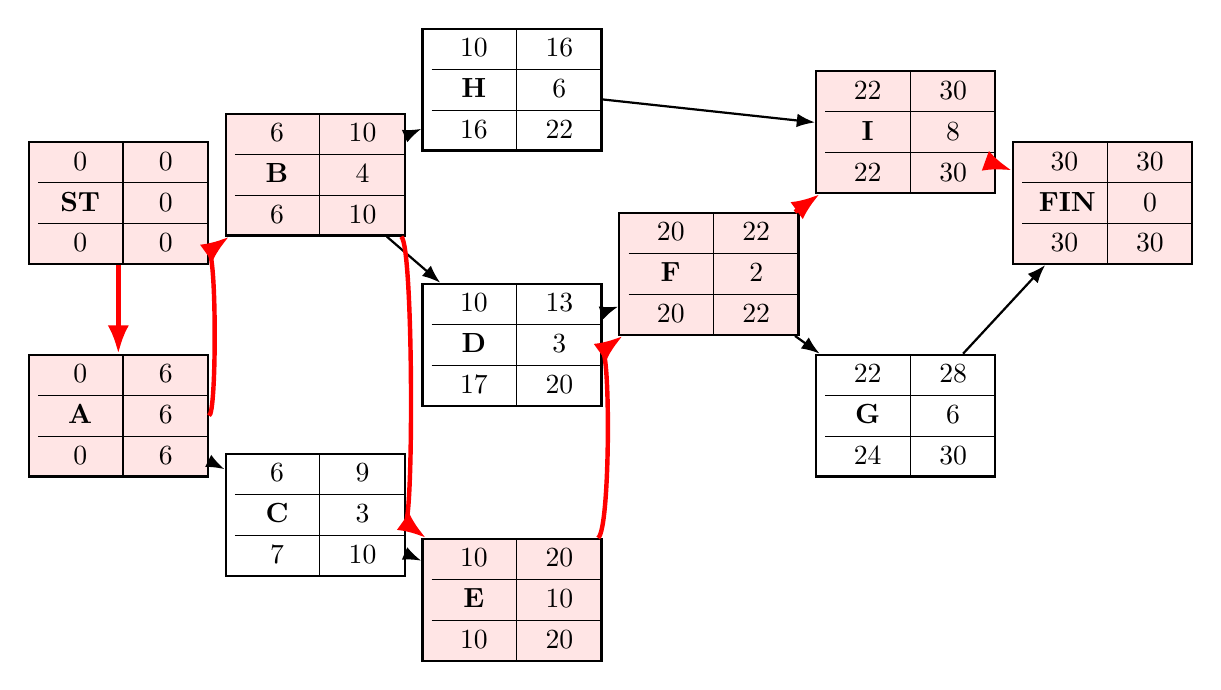
\begin{tikzpicture}[
        myarrow/.style={-Latex, thick},
        cparrow/.style={-Latex, ultra thick, red},
        x=2.5cm, y=1.8cm
    ]
    % Coordinates
    \coordinate (posST) at (0, 1);
    \coordinate (posA)  at (0, -0.5);
    \coordinate (posB)  at (1, 1.2);
    \coordinate (posC)  at (1, -1.2);
    \coordinate (posH)  at (2, 1.8);
    \coordinate (posD)  at (2, 0);
    \coordinate (posE)  at (2, -1.8);
    \coordinate (posI)  at (4, 1.5);
    \coordinate (posF)  at (3, 0.5);
    \coordinate (posG)  at (4, -0.5);
    \coordinate (posFIN) at (5, 1);

    \cpmnode{fill=red!10}{ST}{(posST)}{0}{0}{ST}{0}{0}{0}
    \cpmnode{fill=red!10}{A}{(posA)}{0}{6}{A}{6}{0}{6}
    \cpmnode{fill=red!10}{B}{(posB)}{6}{10}{B}{4}{6}{10}
    \cpmnode{fill=white}{C}{(posC)}{6}{9}{C}{3}{7}{10}
    \cpmnode{fill=white}{H}{(posH)}{10}{16}{H}{6}{16}{22}
    \cpmnode{fill=white}{D}{(posD)}{10}{13}{D}{3}{17}{20}
    \cpmnode{fill=red!10}{E}{(posE)}{10}{20}{E}{10}{10}{20}
    \cpmnode{fill=red!10}{F}{(posF)}{20}{22}{F}{2}{20}{22}
    \cpmnode{fill=white}{G}{(posG)}{22}{28}{G}{6}{24}{30}
    \cpmnode{fill=red!10}{I}{(posI)}{22}{30}{I}{8}{22}{30}
    \cpmnode{fill=red!10}{FIN}{(posFIN)}{30}{30}{FIN}{0}{30}{30}
    \draw[cparrow] (ST) .. controls ++(0,-0.5) and ++(0,0.5) .. (A);
    \draw[cparrow] (A) .. controls ++(0.5,0) and ++(-0.5,-0.5) .. (B);
    \draw[myarrow] (A) -- (C);
    \draw[myarrow] (B) -- (H);
    \draw[myarrow] (B) -- (D);
    \draw[cparrow] (B) .. controls ++(0.5,-0.5) and ++(-0.5,0.5) .. (E);
    \draw[myarrow] (C) -- (E);
    \draw[myarrow] (D) -- (F);
    \draw[cparrow] (E) .. controls ++(0.5,0.5) and ++(-0.5,-0.5) .. (F);
    \draw[myarrow] (H) -- (I);
    \draw[cparrow] (F) .. controls ++(0.5,0.5) and ++(-0.5,-0.5) .. (I);
    \draw[myarrow] (F) -- (G);
    \draw[cparrow] (I) -- (FIN);
    \draw[myarrow] (G) -- (FIN);
    \end{tikzpicture}
    \end{adjustbox}
    \vspace{0.5em}
    \begin{center}
    \Large \textcolor{red}{\textbf{Critical Path: Start - A - B - E - F - I - Finish}}
    \end{center}
\end{frame}

\begin{frame}{Time-Cost Tradeoffs -- Crashing Activities}
    The management of AeroTech Solutions is giving some thoughts to putting extra resources into the project so that it can be completed within \textbf{26 weeks}. Each activity has been studied, and a set of \underline{crash times} (in weeks) and cost has been developed. \underline{Determine a crash plan which minimizes the total cost of completing the project within 26 weeks.}
    
    \vspace{0.5em}
    \begin{alertblock}{Connection to Simulation}
        When you decide to authorize overtime, hire more staff, or outsource to hit a looming deadline, you are effectively \textbf{``crashing''} the project. You must weigh the \textbf{cost per week saved}.
    \end{alertblock}
    
    \vspace{0.5em}
    \begin{adjustbox}{max width=\linewidth, max height=0.45\textheight, center}
    \begin{tabular}{llcccc}
        \toprule
        \textbf{Activity} & \textbf{Activity Description} & \textbf{Normal} & \textbf{Normal} & \textbf{Crash} & \textbf{Crash} \\
        & & \textbf{Time} & \textbf{Cost} & \textbf{Time} & \textbf{Cost} \\
        \midrule
        A & Conduct market analysis & 6 & \$240,000 & 5 & \$300,000 \\
        B & Secure manufacturing facilities & 4 & \$300,000 & 3 & \$400,000 \\
        C & Hire production managers & 3 & \$150,000 & 2 & \$240,000 \\
        D & Procure raw materials & 3 & \$540,000 & 2 & \$750,000 \\
        E & Hire \& train assembly team & 10 & \$900,000 & 7 & \$1,440,000 \\
        F & Manufacture pilot units & 2 & \$300,000 & 1 & \$390,000 \\
        G & Scale to full production & 6 & \$1,350,000 & 4 & \$3,200,000 \\
        H & Develop marketing strategy & 6 & \$450,000 & 3 & \$900,000 \\
        I & Execute global launch campaign & 8 & \$1,050,000 & 4 & \$2,600,000 \\
        \bottomrule
    \end{tabular}
    \end{adjustbox}
\end{frame}

\begin{frame}{A Heuristic Approach}
    \textbf{What activities to crash and how much to crash?}
    
    \vspace{0.5em}
    \begin{adjustbox}{max width=\linewidth, max height=0.6\textheight, center}
    \begin{tabular}{ccrrccc>{\columncolor{green!40}}c}
        \toprule
        \textbf{Act.} & \textbf{Time} & \textbf{Budgeted} & \textbf{Crash} & $\Delta$\textbf{Cost} & $\Delta$\textbf{Time} & \textbf{Crash Cost / Wk} & \textbf{Slack} \\
        & $(T_i)$ & \textbf{Cost} $(C_i)$ & \textbf{Cost} $(C'_i)$ & $(C'_i - C_i)$ & $(T_i - T'_i)$ & $(\Delta C / \Delta T)$ & \text{(From CPM)} \\
        \midrule
        A & 6 & \$240,000 & \$300,000 & \$60,000 & 1 & \$60,000 & 0 \\
        B & 4 & \$300,000 & \$400,000 & \$100,000 & 1 & \$100,000 & 0 \\
        C & 3 & \$150,000 & \$240,000 & \$90,000 & 1 & \$90,000 & 1 \\
        D & 3 & \$540,000 & \$750,000 & \$210,000 & 1 & \$210,000 & 7 \\
        E & 10 & \$900,000 & \$1,440,000 & \$540,000 & 3 & \$180,000 & 0 \\
        F & 2 & \$300,000 & \$390,000 & \$90,000 & 1 & \$90,000 & 0 \\
        G & 6 & \$1,350,000 & \$3,200,000 & \$1,850,000 & 2 & \$925,000 & 2 \\
        H & 6 & \$450,000 & \$900,000 & \$450,000 & 3 & \$150,000 & 6 \\
        I & 8 & \$1,050,000 & \$2,600,000 & \$1,550,000 & 4 & \$387,500 & 0 \\
        \bottomrule
    \end{tabular}
    \end{adjustbox}
    
    \vspace{0.5em}
    \small Current Critical Path: A - B - E - F - I (30 weeks)\\
    Need completion in 26 weeks.
\end{frame}

\begin{frame}{Crashing Step 1: Crash Activity A by 1 Week}
    \begin{columns}[T]
    \begin{column}{0.4\textwidth}
        \small
        \begin{itemize}
            \item Activity A is on the critical path and has the lowest Crash Cost / Week (\$60,000).
            \item New Duration for A = 5.
            \item Entire project duration drops to \textbf{29 weeks}.
        \end{itemize}
        \vspace{1em}
        \textbf{Next:} Which activity to crash next?
        \begin{itemize}
            \item Check critical path. It remains \textbf{A-B-E-F-I}.
            \item Next cheapest on CP is F (\$90k/wk).
        \end{itemize}
    \end{column}
    \begin{column}{0.6\textwidth}
        \begin{adjustbox}{max width=\linewidth, max height=0.75\textheight, center}
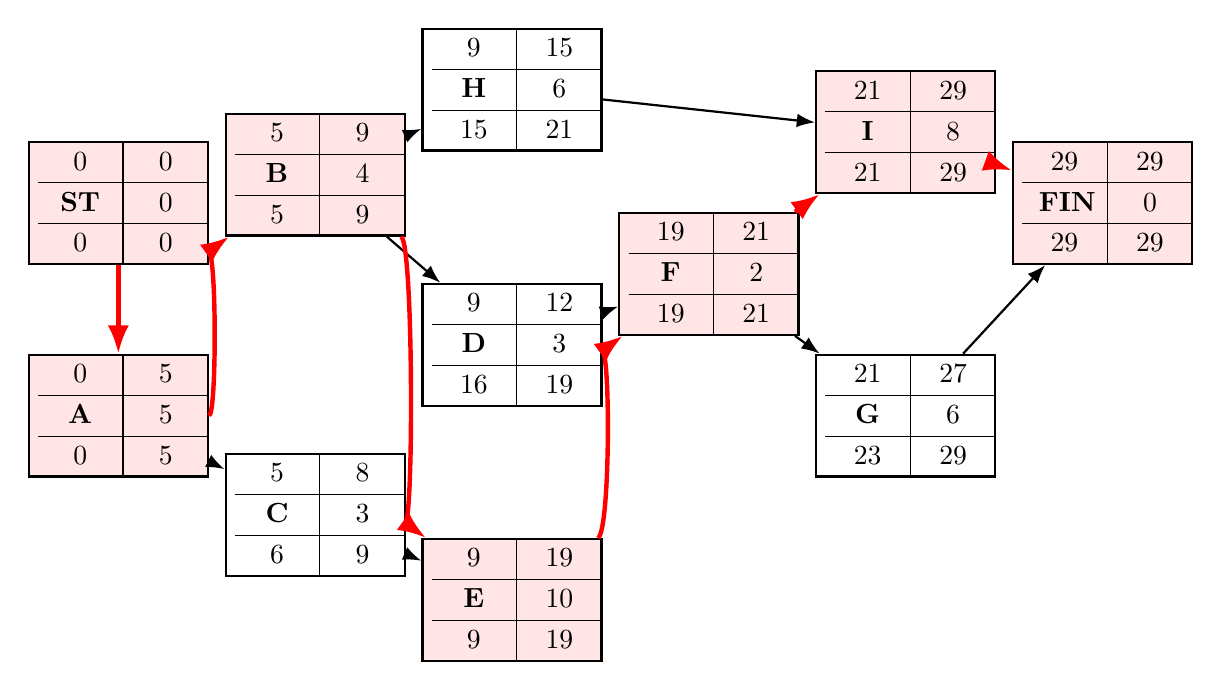
\begin{tikzpicture}[
        myarrow/.style={-Latex, thick},
        cparrow/.style={-Latex, ultra thick, red},
        x=2.5cm, y=1.8cm
    ]
    % Coordinates
    \coordinate (posST) at (0, 1);
    \coordinate (posA)  at (0, -0.5);
    \coordinate (posB)  at (1, 1.2);
    \coordinate (posC)  at (1, -1.2);
    \coordinate (posH)  at (2, 1.8);
    \coordinate (posD)  at (2, 0);
    \coordinate (posE)  at (2, -1.8);
    \coordinate (posI)  at (4, 1.5);
    \coordinate (posF)  at (3, 0.5);
    \coordinate (posG)  at (4, -0.5);
    \coordinate (posFIN) at (5, 1);

    \cpmnode{fill=red!10}{ST}{(posST)}{0}{0}{ST}{0}{0}{0}
    \cpmnode{fill=red!10}{A}{(posA)}{0}{5}{A}{5}{0}{5}
    \cpmnode{fill=red!10}{B}{(posB)}{5}{9}{B}{4}{5}{9}
    \cpmnode{fill=white}{C}{(posC)}{5}{8}{C}{3}{6}{9}
    \cpmnode{fill=white}{H}{(posH)}{9}{15}{H}{6}{15}{21}
    \cpmnode{fill=white}{D}{(posD)}{9}{12}{D}{3}{16}{19}
    \cpmnode{fill=red!10}{E}{(posE)}{9}{19}{E}{10}{9}{19}
    \cpmnode{fill=red!10}{F}{(posF)}{19}{21}{F}{2}{19}{21}
    \cpmnode{fill=white}{G}{(posG)}{21}{27}{G}{6}{23}{29}
    \cpmnode{fill=red!10}{I}{(posI)}{21}{29}{I}{8}{21}{29}
    \cpmnode{fill=red!10}{FIN}{(posFIN)}{29}{29}{FIN}{0}{29}{29}
    \draw[cparrow] (ST) .. controls ++(0,-0.5) and ++(0,0.5) .. (A);
    \draw[cparrow] (A) .. controls ++(0.5,0) and ++(-0.5,-0.5) .. (B);
    \draw[myarrow] (A) -- (C);
    \draw[myarrow] (B) -- (H);
    \draw[myarrow] (B) -- (D);
    \draw[cparrow] (B) .. controls ++(0.5,-0.5) and ++(-0.5,0.5) .. (E);
    \draw[myarrow] (C) -- (E);
    \draw[myarrow] (D) -- (F);
    \draw[cparrow] (E) .. controls ++(0.5,0.5) and ++(-0.5,-0.5) .. (F);
    \draw[myarrow] (H) -- (I);
    \draw[cparrow] (F) .. controls ++(0.5,0.5) and ++(-0.5,-0.5) .. (I);
    \draw[myarrow] (F) -- (G);
    \draw[cparrow] (I) -- (FIN);
    \draw[myarrow] (G) -- (FIN);
    \end{tikzpicture}
        \end{adjustbox}
    \end{column}
    \end{columns}
\end{frame}

\begin{frame}{Crashing Step 2: Crash Activity F by 1 Week}
    \begin{columns}[T]
    \begin{column}{0.4\textwidth}
        \small
        \begin{itemize}
            \item Crash F by 1 week. Cost = \$90,000.
            \item New Duration for F = 1.
            \item Entire project duration drops to \textbf{28 weeks}.
        \end{itemize}
        \vspace{1em}
        \textbf{Next:} Which activity to crash next?
        \begin{itemize}
            \item Check critical path. It remains \textbf{A-B-E-F-I}.
            \item Next cheapest on CP is B (\$100k/wk).
        \end{itemize}
    \end{column}
    \begin{column}{0.6\textwidth}
        \begin{adjustbox}{max width=\linewidth, max height=0.75\textheight, center}
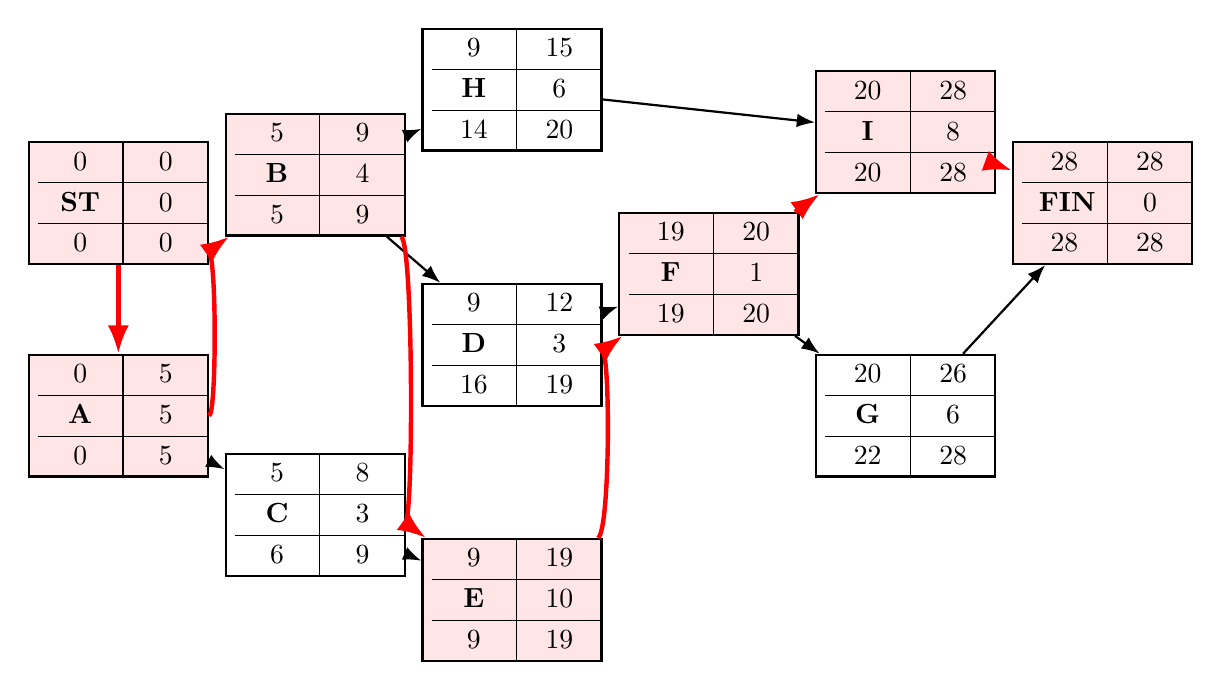
\begin{tikzpicture}[
        myarrow/.style={-Latex, thick},
        cparrow/.style={-Latex, ultra thick, red},
        x=2.5cm, y=1.8cm
    ]
    % Coordinates
    \coordinate (posST) at (0, 1);
    \coordinate (posA)  at (0, -0.5);
    \coordinate (posB)  at (1, 1.2);
    \coordinate (posC)  at (1, -1.2);
    \coordinate (posH)  at (2, 1.8);
    \coordinate (posD)  at (2, 0);
    \coordinate (posE)  at (2, -1.8);
    \coordinate (posI)  at (4, 1.5);
    \coordinate (posF)  at (3, 0.5);
    \coordinate (posG)  at (4, -0.5);
    \coordinate (posFIN) at (5, 1);

    \cpmnode{fill=red!10}{ST}{(posST)}{0}{0}{ST}{0}{0}{0}
    \cpmnode{fill=red!10}{A}{(posA)}{0}{5}{A}{5}{0}{5}
    \cpmnode{fill=red!10}{B}{(posB)}{5}{9}{B}{4}{5}{9}
    \cpmnode{fill=white}{C}{(posC)}{5}{8}{C}{3}{6}{9}
    \cpmnode{fill=white}{H}{(posH)}{9}{15}{H}{6}{14}{20}
    \cpmnode{fill=white}{D}{(posD)}{9}{12}{D}{3}{16}{19}
    \cpmnode{fill=red!10}{E}{(posE)}{9}{19}{E}{10}{9}{19}
    \cpmnode{fill=red!10}{F}{(posF)}{19}{20}{F}{1}{19}{20}
    \cpmnode{fill=white}{G}{(posG)}{20}{26}{G}{6}{22}{28}
    \cpmnode{fill=red!10}{I}{(posI)}{20}{28}{I}{8}{20}{28}
    \cpmnode{fill=red!10}{FIN}{(posFIN)}{28}{28}{FIN}{0}{28}{28}
    \draw[cparrow] (ST) .. controls ++(0,-0.5) and ++(0,0.5) .. (A);
    \draw[cparrow] (A) .. controls ++(0.5,0) and ++(-0.5,-0.5) .. (B);
    \draw[myarrow] (A) -- (C);
    \draw[myarrow] (B) -- (H);
    \draw[myarrow] (B) -- (D);
    \draw[cparrow] (B) .. controls ++(0.5,-0.5) and ++(-0.5,0.5) .. (E);
    \draw[myarrow] (C) -- (E);
    \draw[myarrow] (D) -- (F);
    \draw[cparrow] (E) .. controls ++(0.5,0.5) and ++(-0.5,-0.5) .. (F);
    \draw[myarrow] (H) -- (I);
    \draw[cparrow] (F) .. controls ++(0.5,0.5) and ++(-0.5,-0.5) .. (I);
    \draw[myarrow] (F) -- (G);
    \draw[cparrow] (I) -- (FIN);
    \draw[myarrow] (G) -- (FIN);
    \end{tikzpicture}
        \end{adjustbox}
    \end{column}
    \end{columns}
\end{frame}

\begin{frame}{Crashing Step 3: Crash Activity B by 1 Week}
    \begin{columns}[T]
    \begin{column}{0.4\textwidth}
        \small
        \begin{itemize}
            \item Crash B by 1 week. Cost = \$100,000.
            \item New Duration for B = 3.
            \item Entire project duration drops to \textbf{27 weeks}.
        \end{itemize}
        \vspace{1em}
        \textbf{Next:} Which activity to crash next?
        \begin{itemize}
            \item Check critical path. It is STILL A-B-E-F-I.
            \item But wait, Activity C's slack has dropped to 0!
            \item We now have \textbf{two} critical paths: \textbf{A-B-E-F-I} and \textbf{A-C-E-F-I}.
        \end{itemize}
    \end{column}
    \begin{column}{0.6\textwidth}
        \begin{adjustbox}{max width=\linewidth, max height=0.75\textheight, center}
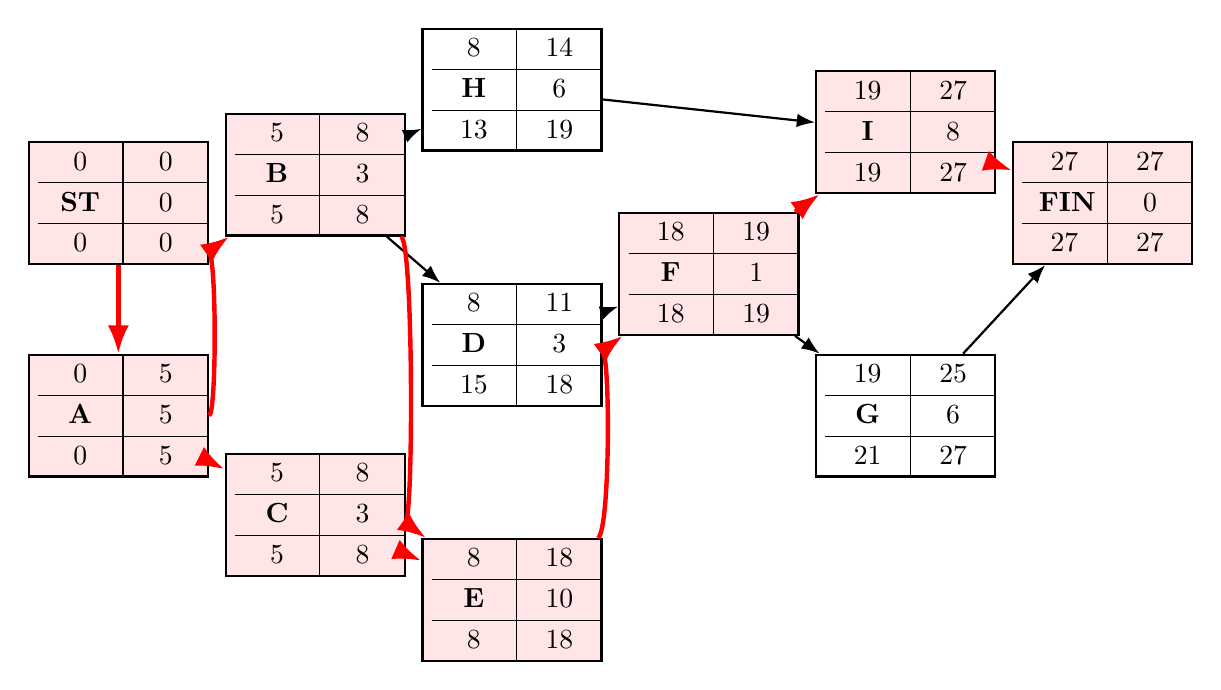
\begin{tikzpicture}[
        myarrow/.style={-Latex, thick},
        cparrow/.style={-Latex, ultra thick, red},
        x=2.5cm, y=1.8cm
    ]
    % Coordinates
    \coordinate (posST) at (0, 1);
    \coordinate (posA)  at (0, -0.5);
    \coordinate (posB)  at (1, 1.2);
    \coordinate (posC)  at (1, -1.2);
    \coordinate (posH)  at (2, 1.8);
    \coordinate (posD)  at (2, 0);
    \coordinate (posE)  at (2, -1.8);
    \coordinate (posI)  at (4, 1.5);
    \coordinate (posF)  at (3, 0.5);
    \coordinate (posG)  at (4, -0.5);
    \coordinate (posFIN) at (5, 1);

    \cpmnode{fill=red!10}{ST}{(posST)}{0}{0}{ST}{0}{0}{0}
    \cpmnode{fill=red!10}{A}{(posA)}{0}{5}{A}{5}{0}{5}
    \cpmnode{fill=red!10}{B}{(posB)}{5}{8}{B}{3}{5}{8}
    \cpmnode{fill=red!10}{C}{(posC)}{5}{8}{C}{3}{5}{8}
    \cpmnode{fill=white}{H}{(posH)}{8}{14}{H}{6}{13}{19}
    \cpmnode{fill=white}{D}{(posD)}{8}{11}{D}{3}{15}{18}
    \cpmnode{fill=red!10}{E}{(posE)}{8}{18}{E}{10}{8}{18}
    \cpmnode{fill=red!10}{F}{(posF)}{18}{19}{F}{1}{18}{19}
    \cpmnode{fill=white}{G}{(posG)}{19}{25}{G}{6}{21}{27}
    \cpmnode{fill=red!10}{I}{(posI)}{19}{27}{I}{8}{19}{27}
    \cpmnode{fill=red!10}{FIN}{(posFIN)}{27}{27}{FIN}{0}{27}{27}
    \draw[cparrow] (ST) .. controls ++(0,-0.5) and ++(0,0.5) .. (A);
    \draw[cparrow] (A) .. controls ++(0.5,0) and ++(-0.5,-0.5) .. (B);
    \draw[cparrow] (A) -- (C);
    \draw[myarrow] (B) -- (H);
    \draw[myarrow] (B) -- (D);
    \draw[cparrow] (B) .. controls ++(0.5,-0.5) and ++(-0.5,0.5) .. (E);
    \draw[cparrow] (C) -- (E);
    \draw[myarrow] (D) -- (F);
    \draw[cparrow] (E) .. controls ++(0.5,0.5) and ++(-0.5,-0.5) .. (F);
    \draw[myarrow] (H) -- (I);
    \draw[cparrow] (F) .. controls ++(0.5,0.5) and ++(-0.5,-0.5) .. (I);
    \draw[myarrow] (F) -- (G);
    \draw[cparrow] (I) -- (FIN);
    \draw[myarrow] (G) -- (FIN);
    \end{tikzpicture}
        \end{adjustbox}
    \end{column}
    \end{columns}
\end{frame}

\begin{frame}{Crashing Step 4: What if we crash C?}
    \begin{columns}[T]
    \begin{column}{0.4\textwidth}
        \small
        \begin{itemize}
            \item If we crash C (cost \$90,000/wk)...
            \item \textbf{Doesn't help.} Because activity E cannot start until \emph{both} B and C finish.
            \item B is 3 weeks, C is 2 weeks. E still waits for B. The total duration remains 27.
            \item To save time, we would have to crash \emph{both} B and C together (cost \$190,000/wk).
        \end{itemize}
    \end{column}
    \begin{column}{0.6\textwidth}
        \begin{adjustbox}{max width=\linewidth, max height=0.75\textheight, center}
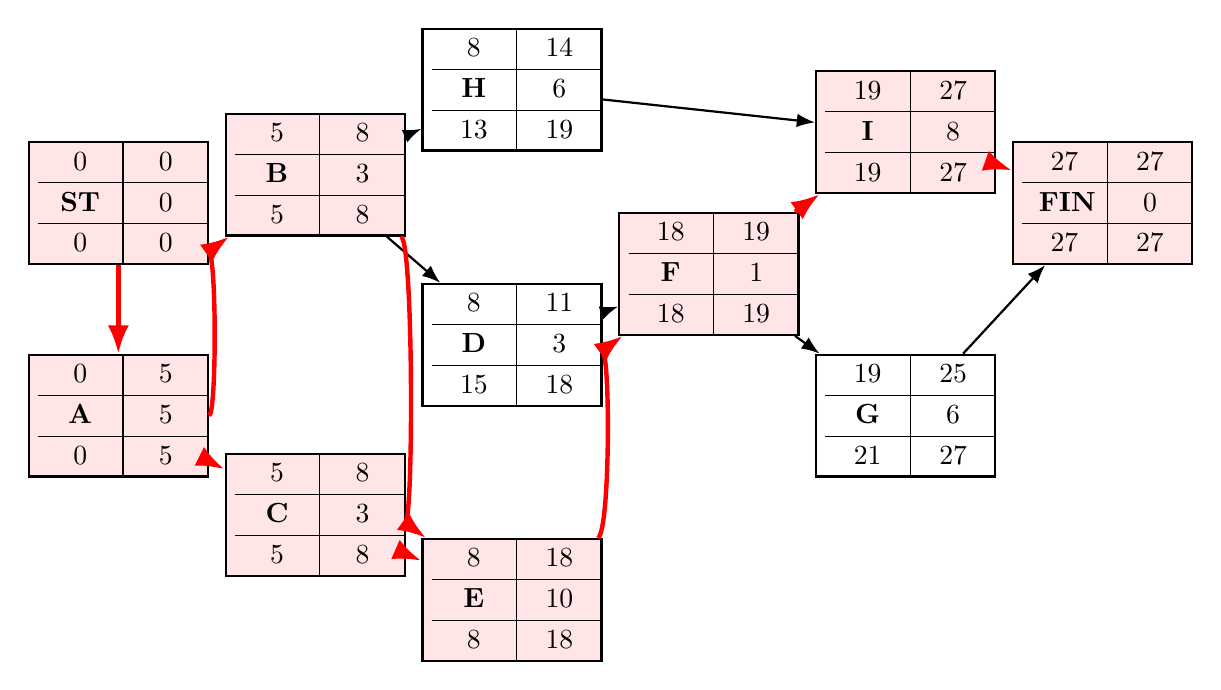
\begin{tikzpicture}[
        myarrow/.style={-Latex, thick},
        cparrow/.style={-Latex, ultra thick, red},
        x=2.5cm, y=1.8cm
    ]
    % Coordinates
    \coordinate (posST) at (0, 1);
    \coordinate (posA)  at (0, -0.5);
    \coordinate (posB)  at (1, 1.2);
    \coordinate (posC)  at (1, -1.2);
    \coordinate (posH)  at (2, 1.8);
    \coordinate (posD)  at (2, 0);
    \coordinate (posE)  at (2, -1.8);
    \coordinate (posI)  at (4, 1.5);
    \coordinate (posF)  at (3, 0.5);
    \coordinate (posG)  at (4, -0.5);
    \coordinate (posFIN) at (5, 1);

    \cpmnode{fill=red!10}{ST}{(posST)}{0}{0}{ST}{0}{0}{0}
    \cpmnode{fill=red!10}{A}{(posA)}{0}{5}{A}{5}{0}{5}
    \cpmnode{fill=red!10}{B}{(posB)}{5}{8}{B}{3}{5}{8}
    \cpmnode{fill=red!10}{C}{(posC)}{5}{8}{C}{3}{5}{8}
    \cpmnode{fill=white}{H}{(posH)}{8}{14}{H}{6}{13}{19}
    \cpmnode{fill=white}{D}{(posD)}{8}{11}{D}{3}{15}{18}
    \cpmnode{fill=red!10}{E}{(posE)}{8}{18}{E}{10}{8}{18}
    \cpmnode{fill=red!10}{F}{(posF)}{18}{19}{F}{1}{18}{19}
    \cpmnode{fill=white}{G}{(posG)}{19}{25}{G}{6}{21}{27}
    \cpmnode{fill=red!10}{I}{(posI)}{19}{27}{I}{8}{19}{27}
    \cpmnode{fill=red!10}{FIN}{(posFIN)}{27}{27}{FIN}{0}{27}{27}
    \draw[cparrow] (ST) .. controls ++(0,-0.5) and ++(0,0.5) .. (A);
    \draw[cparrow] (A) .. controls ++(0.5,0) and ++(-0.5,-0.5) .. (B);
    \draw[cparrow] (A) -- (C);
    \draw[myarrow] (B) -- (H);
    \draw[myarrow] (B) -- (D);
    \draw[cparrow] (B) .. controls ++(0.5,-0.5) and ++(-0.5,0.5) .. (E);
    \draw[cparrow] (C) -- (E);
    \draw[myarrow] (D) -- (F);
    \draw[cparrow] (E) .. controls ++(0.5,0.5) and ++(-0.5,-0.5) .. (F);
    \draw[myarrow] (H) -- (I);
    \draw[cparrow] (F) .. controls ++(0.5,0.5) and ++(-0.5,-0.5) .. (I);
    \draw[myarrow] (F) -- (G);
    \draw[cparrow] (I) -- (FIN);
    \draw[myarrow] (G) -- (FIN);
    \end{tikzpicture}
        \end{adjustbox}
    \end{column}
    \end{columns}
\end{frame}

\begin{frame}{Crashing Step 5: Crash Activity E by 1 Week}
    \begin{columns}[T]
    \begin{column}{0.4\textwidth}
        \small
        \begin{itemize}
            \item Instead of crashing B and C, crash E.
            \item E is on \emph{both} critical paths!
            \item Crash E by 1 week. Cost = \$180,000.
            \item New Duration for E = 9.
            \item Entire project duration drops to \textbf{26 weeks}!
        \end{itemize}
        \vspace{1em}
        \textbf{Success!} We achieved 26 weeks.
    \end{column}
    \begin{column}{0.6\textwidth}
        \begin{adjustbox}{max width=\linewidth, max height=0.75\textheight, center}
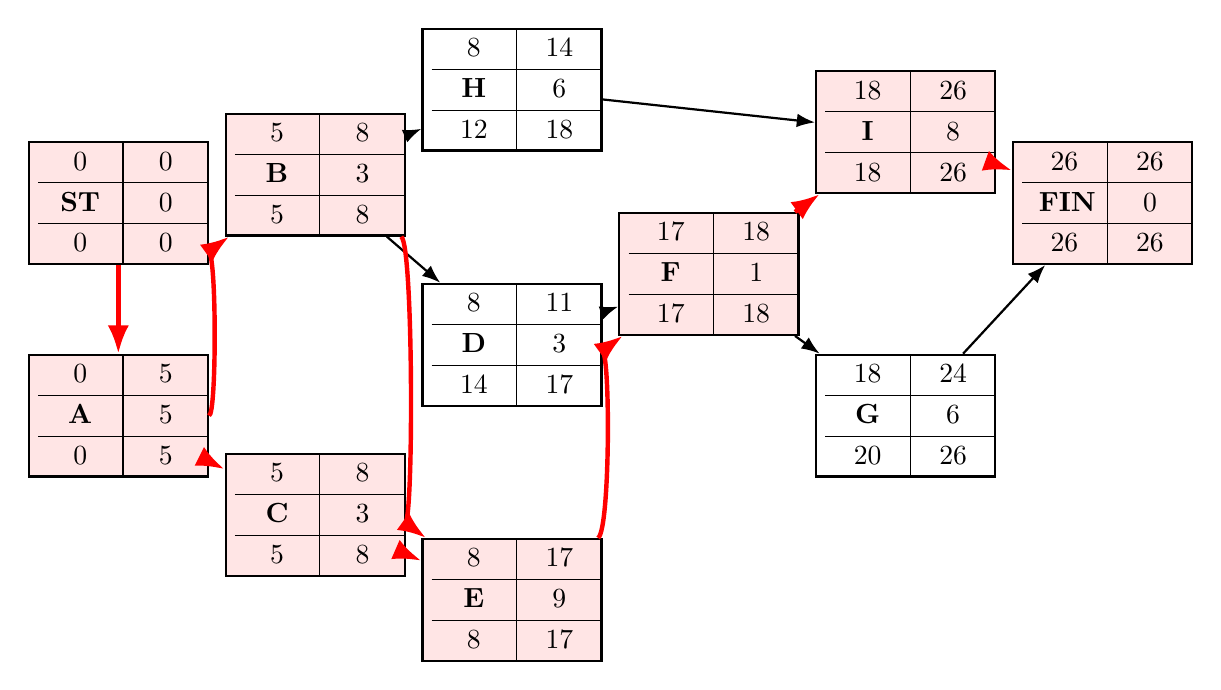
\begin{tikzpicture}[
        myarrow/.style={-Latex, thick},
        cparrow/.style={-Latex, ultra thick, red},
        x=2.5cm, y=1.8cm
    ]
    % Coordinates
    \coordinate (posST) at (0, 1);
    \coordinate (posA)  at (0, -0.5);
    \coordinate (posB)  at (1, 1.2);
    \coordinate (posC)  at (1, -1.2);
    \coordinate (posH)  at (2, 1.8);
    \coordinate (posD)  at (2, 0);
    \coordinate (posE)  at (2, -1.8);
    \coordinate (posI)  at (4, 1.5);
    \coordinate (posF)  at (3, 0.5);
    \coordinate (posG)  at (4, -0.5);
    \coordinate (posFIN) at (5, 1);

    \cpmnode{fill=red!10}{ST}{(posST)}{0}{0}{ST}{0}{0}{0}
    \cpmnode{fill=red!10}{A}{(posA)}{0}{5}{A}{5}{0}{5}
    \cpmnode{fill=red!10}{B}{(posB)}{5}{8}{B}{3}{5}{8}
    \cpmnode{fill=red!10}{C}{(posC)}{5}{8}{C}{3}{5}{8}
    \cpmnode{fill=white}{H}{(posH)}{8}{14}{H}{6}{12}{18}
    \cpmnode{fill=white}{D}{(posD)}{8}{11}{D}{3}{14}{17}
    \cpmnode{fill=red!10}{E}{(posE)}{8}{17}{E}{9}{8}{17}
    \cpmnode{fill=red!10}{F}{(posF)}{17}{18}{F}{1}{17}{18}
    \cpmnode{fill=white}{G}{(posG)}{18}{24}{G}{6}{20}{26}
    \cpmnode{fill=red!10}{I}{(posI)}{18}{26}{I}{8}{18}{26}
    \cpmnode{fill=red!10}{FIN}{(posFIN)}{26}{26}{FIN}{0}{26}{26}
    \draw[cparrow] (ST) .. controls ++(0,-0.5) and ++(0,0.5) .. (A);
    \draw[cparrow] (A) .. controls ++(0.5,0) and ++(-0.5,-0.5) .. (B);
    \draw[cparrow] (A) -- (C);
    \draw[myarrow] (B) -- (H);
    \draw[myarrow] (B) -- (D);
    \draw[cparrow] (B) .. controls ++(0.5,-0.5) and ++(-0.5,0.5) .. (E);
    \draw[cparrow] (C) -- (E);
    \draw[myarrow] (D) -- (F);
    \draw[cparrow] (E) .. controls ++(0.5,0.5) and ++(-0.5,-0.5) .. (F);
    \draw[myarrow] (H) -- (I);
    \draw[cparrow] (F) .. controls ++(0.5,0.5) and ++(-0.5,-0.5) .. (I);
    \draw[myarrow] (F) -- (G);
    \draw[cparrow] (I) -- (FIN);
    \draw[myarrow] (G) -- (FIN);
    \end{tikzpicture}
        \end{adjustbox}
    \end{column}
    \end{columns}
\end{frame}

\begin{frame}{About Heuristic Approach}
    \begin{itemize}[<+->]
        \item \textbf{Remember:}
        \begin{itemize}
            \item As you crash the current critical activities, \underline{other paths may become critical}.
        \end{itemize}
        \vspace{1em}
        \item \textbf{Recommendation:}
        \begin{itemize}
            \item Crash activities \underline{one by one}.
            \item After crashing one activity, check the \underline{critical path(s)} in the revised network.
        \end{itemize}
    \end{itemize}
\end{frame}

\begin{frame}{Project Scheduling with Uncertain Activity Times}
    The R\&D team at AeroTech used a completely new AI navigation chip for the drone. Given the massive market hype, management wants to roll out the product as soon as possible. However, due to supply chain complexities and new manufacturing techniques, the operations managers can only give a rough estimate (optimistic, most probable, pessimistic) on the duration time of activities. \textbf{What would be the expected time required to complete the project?}
    
    \vspace{0.5em}
    \begin{alertblock}{Connection to Simulation}
        In the game, you will face unexpected curveballs (e.g., staff quitting, tech failures). PERT proves mathematically why a single deterministic plan is an illusion, and why you must manage risk dynamically.
    \end{alertblock}
    
    \begin{adjustbox}{max width=\linewidth, max height=0.25\textheight, center}
    \begin{tabular}{cccc}
        \toprule
        \textbf{Activity} & \textbf{Optimistic ($a_i$)} & \textbf{Most Probable ($m_i$)} & \textbf{Pessimistic ($b_i$)} \\
        \midrule
        A & 4 & 6 & 7 \\
        B & 4 & 6 & 9 \\
        \dots & \dots & \dots & \dots \\
        \bottomrule
    \end{tabular}
    \end{adjustbox}
\end{frame}

\begin{frame}{Three-Point Estimation Technique (PERT)}
    \textbf{A. Time estimates}
    \begin{enumerate}
        \item For each activity, estimate:
        \begin{itemize}
            \item $a_i$ = optimistic time
            \item $b_i$ = pessimistic time
            \item $m_i$ = most probable time
        \end{itemize}
        \item Compute approximate value assuming a beta probability distribution:
    \end{enumerate}
    
    \vspace{1em}
    \begin{block}{}
        \centering
        Expected Time = $\mu_i = \frac{a_i + 4m_i + b_i}{6}$
    \end{block}
    
    \begin{block}{}
        \centering
        Variance = $\sigma_i^2 = \left(\frac{b_i - a_i}{6}\right)^2$
    \end{block}
\end{frame}

\begin{frame}{Critical Path \& Probabilistic Analysis}
    \textbf{B. Procedure}
    \begin{enumerate}
        \item Treat the \underline{expected activity times} as the known duration of activity. Use the PERT/CPM procedure to \underline{find the critical path} of the project.
        \item Compute estimates of \underline{mean and variance of project} completion time as sum of expected times and variances along critical path:
        \begin{itemize}
            \item Mean ($\mu$) = Sum of Expected Times on Critical Path
            \item Variance ($\sigma^2$) = Sum of Variances on Critical Path
        \end{itemize}
        \item Assume the project completion time is normally distributed $N(\mu, \sigma)$
        \item Use Standardized Normal Distribution Table to determine certainty of completing project within a given time frame.
    \end{enumerate}
\end{frame}

\begin{frame}{AeroTech PERT Calculations}
    \begin{adjustbox}{max width=\linewidth, max height=0.65\textheight, center}
    \begin{tabular}{ccccccc}
        \toprule
        & \textbf{Activity} & \textbf{Optimistic} & \textbf{Most Prob.} & \textbf{Pessimistic} & \textbf{Mean Time ($\mu_i$)} & \textbf{Variance ($\sigma_i^2$)} \\
        \midrule
        \checkmark & A & 4 & 6 & 7 & 5.83 & 0.25 \\
        \checkmark & B & 4 & 6 & 9 & 6.17 & 0.69 \\
        & C & 3 & 4 & 5 & 4 & 0.11 \\
        & D & 3 & 5 & 7 & 5 & 0.44 \\
        \checkmark & E & 10 & 14 & 16 & 13.67 & 1 \\
        \checkmark & F & 2 & 2 & 3 & 2.17 & 0.03 \\
        \checkmark & G & 6 & 8 & 12 & 8.33 & 1 \\
        & H & 4 & 6 & 7 & 5.83 & 0.25 \\
        & I & 6 & 8 & 9 & 7.83 & 0.25 \\
        \bottomrule
    \end{tabular}
    \end{adjustbox}
    
    \vspace{1em}
    \textbf{CPM gives Critical Path: A-B-E-F-G}
\end{frame}

\begin{frame}{PERT Network Diagram (Expected Times)}
    \begin{adjustbox}{max width=\linewidth, max height=0.7\textheight, center}
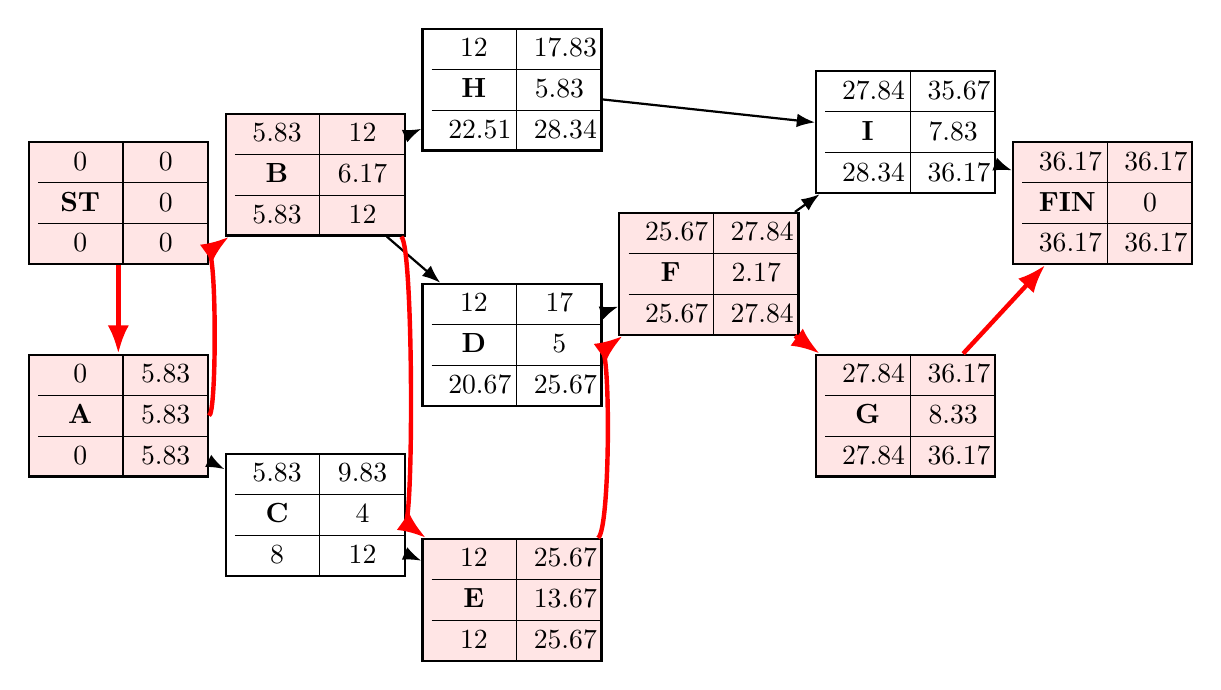
\begin{tikzpicture}[
        myarrow/.style={-Latex, thick},
        cparrow/.style={-Latex, ultra thick, red},
        x=2.5cm, y=1.8cm
    ]
    % Coordinates
    \coordinate (posST) at (0, 1);
    \coordinate (posA)  at (0, -0.5);
    \coordinate (posB)  at (1, 1.2);
    \coordinate (posC)  at (1, -1.2);
    \coordinate (posH)  at (2, 1.8);
    \coordinate (posD)  at (2, 0);
    \coordinate (posE)  at (2, -1.8);
    \coordinate (posI)  at (4, 1.5);
    \coordinate (posF)  at (3, 0.5);
    \coordinate (posG)  at (4, -0.5);
    \coordinate (posFIN) at (5, 1);

    \cpmnode{fill=red!10}{ST}{(posST)}{0}{0}{ST}{0}{0}{0}
    \cpmnode{fill=red!10}{A}{(posA)}{0}{5.83}{A}{5.83}{0}{5.83}
    \cpmnode{fill=red!10}{B}{(posB)}{5.83}{12}{B}{6.17}{5.83}{12}
    \cpmnode{fill=white}{C}{(posC)}{5.83}{9.83}{C}{4}{8}{12}
    \cpmnode{fill=white}{H}{(posH)}{12}{17.83}{H}{5.83}{22.51}{28.34}
    \cpmnode{fill=white}{D}{(posD)}{12}{17}{D}{5}{20.67}{25.67}
    \cpmnode{fill=red!10}{E}{(posE)}{12}{25.67}{E}{13.67}{12}{25.67}
    \cpmnode{fill=red!10}{F}{(posF)}{25.67}{27.84}{F}{2.17}{25.67}{27.84}
    \cpmnode{fill=red!10}{G}{(posG)}{27.84}{36.17}{G}{8.33}{27.84}{36.17}
    \cpmnode{fill=white}{I}{(posI)}{27.84}{35.67}{I}{7.83}{28.34}{36.17}
    \cpmnode{fill=red!10}{FIN}{(posFIN)}{36.17}{36.17}{FIN}{0}{36.17}{36.17}
    \draw[cparrow] (ST) .. controls ++(0,-0.5) and ++(0,0.5) .. (A);
    \draw[cparrow] (A) .. controls ++(0.5,0) and ++(-0.5,-0.5) .. (B);
    \draw[myarrow] (A) -- (C);
    \draw[myarrow] (B) -- (H);
    \draw[myarrow] (B) -- (D);
    \draw[cparrow] (B) .. controls ++(0.5,-0.5) and ++(-0.5,0.5) .. (E);
    \draw[myarrow] (C) -- (E);
    \draw[myarrow] (D) -- (F);
    \draw[cparrow] (E) .. controls ++(0.5,0.5) and ++(-0.5,-0.5) .. (F);
    \draw[myarrow] (H) -- (I);
    \draw[myarrow] (F) .. controls ++(0.5,0.5) and ++(-0.5,-0.5) .. (I);
    \draw[cparrow] (F) -- (G);
    \draw[myarrow] (I) -- (FIN);
    \draw[cparrow] (G) -- (FIN);
    \end{tikzpicture}
    \end{adjustbox}
    \vspace{0.5em}
    \begin{center}
    \Large \textcolor{red}{\textbf{Critical Path: Start - A - B - E - F - G - Finish}}
    \end{center}
\end{frame}

\begin{frame}{Project Completion Probabilities}
    Suppose the critical path is: A - B - E - F - G
    
    \vspace{1em}
    \textbf{(1) What is the estimated expected completion time?}
    \begin{itemize}
        \item $\mu_{CP} = 5.83 + 6.17 + 13.67 + 2.17 + 8.33 = 36.17$
        \item $\sigma_{CP}^2 = 0.25 + 0.69 + 1 + 0.03 + 1 = 2.97$
    \end{itemize}
    
    \vspace{1em}
    \textbf{(2) What is the probability of completing the project in 33 weeks?}
    \begin{itemize}
        \item \texttt{NORM.DIST(33, 36.17, SQRT(2.97), 1) = 0.0329 or 3.3\%}
    \end{itemize}
    
    \vspace{1em}
    \textbf{(3) With 90\% probability, what is the project completion time?}
    \begin{itemize}
        \item \texttt{NORM.INV(0.9, 36.17, SQRT(2.97)) = 38.37 days}
    \end{itemize}
\end{frame}

\section{Simulation Introduction}

\begin{frame}{Putting Theory into Practice: HBS Simulation}
    \begin{itemize}[<+->]
        \item \textbf{The Setup:} You will step into the role of a Project Manager mid-flight.
        \item \textbf{The Goal:} Successfully deliver a competitive product to market in a dynamic, unpredictable environment.
        \item \textbf{The 3 Levers:} Manage \textbf{Scope} dynamically, allocate \textbf{Resources} wisely, and hit \textbf{Schedule} deadlines.
        \item \textbf{The Human Element:} You must also manage team morale, stress, and coordination meetings (standups, coaching).
    \end{itemize}
\end{frame}

\begin{frame}{Scenario A: Realistic Targets}
    \begin{itemize}[<+->]
        \item \textbf{The Situation:} A standard project with realistic targets and relatively low uncertainty.
        \item \textbf{Your Strategy:} 
        \begin{itemize}
            \item What resource choices (team size, skill, overtime, outsourcing) give you the best results?
            \item Do you need prototypes? Why or why not?
            \item Will you ever delay non-critical tasks?
        \end{itemize}
        \vspace{1em}
        \item \textbf{Apply the Class Tools:} How can identifying \textbf{slack} from CPM help you optimize resources in this scenario?
    \end{itemize}
\end{frame}

\begin{frame}{Scenario C: Mid-Project Surprise}
    \begin{itemize}[<+->]
        \item \textbf{The Situation:} A competitor issues a surprise announcement mid-project, abruptly tightening your schedule target.
        \item \textbf{Your Strategy:}
        \begin{itemize}
            \item When the schedule suddenly shrinks, what do you do? Add resources? Cut scope? Authorize more overtime?
            \item What happens to team morale and product quality?
        \end{itemize}
        \vspace{1em}
        \item \textbf{Apply the Class Tools:} How is this like \textbf{crashing} activities after you have already started the project? Did any new activities suddenly become critical?
    \end{itemize}
\end{frame}

\begin{frame}{Connecting the Simulation to Session 3 Tools}
    As you play, keep these three analytical tools in mind:
    \vspace{1em}
    \begin{enumerate}[<+->]
        \item \textbf{CPM \& Critical Path:} Did the critical path change when you made decisions or when surprises occurred?
        \item \textbf{Crashing:} Did adding resources always save time? Or were there hidden costs (Brooks's Law, communication overhead)?
        \item \textbf{PERT / Uncertainty:} How did the surprises in Scenario C feel compared to the mathematical variance ($\sigma^2$) in our PERT activity times?
    \end{enumerate}
    \vspace{1em}
    \pause
    \begin{center}
        \Large \textbf{Let's log in and play!}
    \end{center}
\end{frame}

\end{document}
